\documentclass[tikz,border=10pt]{standalone}
\usepackage{tikz}
\usetikzlibrary{shapes,arrows,positioning,calc,patterns,shadows,arrows.meta}

\definecolor{bertblue}{RGB}{66,133,244}
\definecolor{gptgreen}{RGB}{52,168,83}
\definecolor{padgray}{RGB}{200,200,200}
\definecolor{realtoken}{RGB}{255,255,255}
\definecolor{sepviolet}{RGB}{142,36,245}
\definecolor{clsorange}{RGB}{251,188,5}

\begin{document}
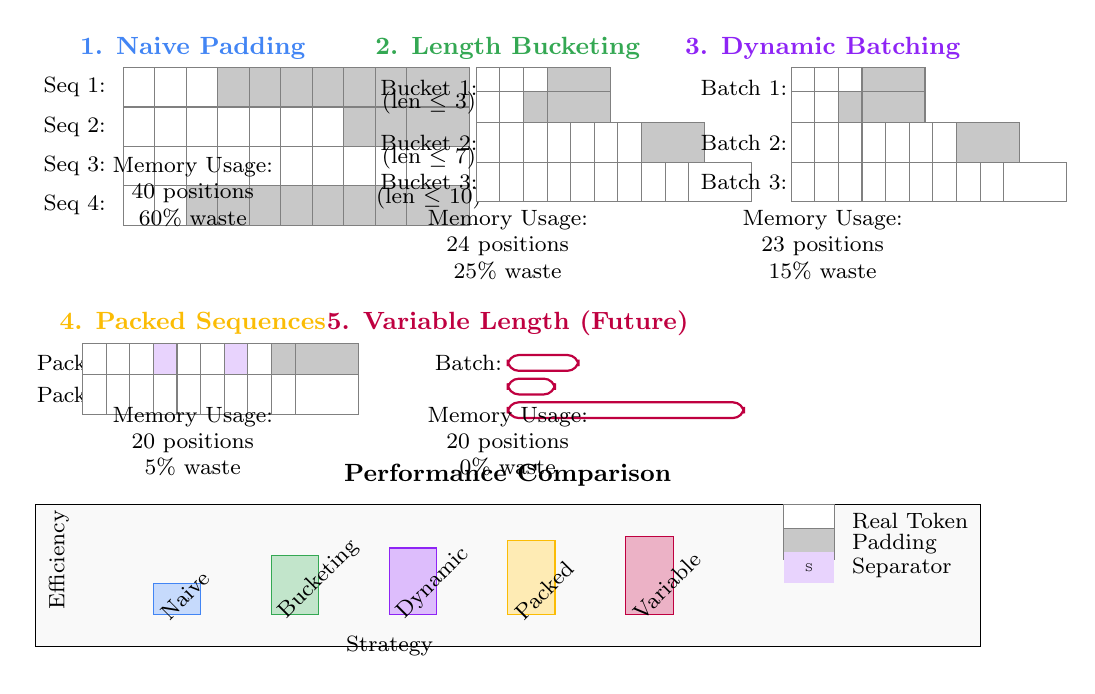
\begin{tikzpicture}[
    token/.style={rectangle, minimum width=0.8cm, minimum height=0.5cm, font=\tiny},
    realtoken/.style={token, fill=realtoken, draw=black!50},
    padtoken/.style={token, fill=padgray, draw=black!50},
    label/.style={font=\footnotesize},
    title/.style={font=\small\bfseries}
]

% === SPACING AND ALIGNMENT DOCUMENTATION ===
% Strategy headers: y=8, x positions at 2, 6, 10
% Sequence rows: y=7.5, 7.0, 6.5, 6.0 with 0.5cm spacing
% Token boxes: 0.4cm horizontal spacing for naive, 0.3cm for others
% Memory usage: y=5.3 and 5.5
% Performance chart: y=1.5, height proportional to efficiency
% Legend: bottom right at x=10.5-11.2

% Strategy 1: Naive Padding
\node[title, bertblue] (naive-title) at (2, 8) {1. Naive Padding};

% Sequences with different lengths - using consistent positioning
\node[label] (seq1-label) at (0.5, 7.5) {Seq 1:};
\foreach \i in {0,...,2} {
    \node[realtoken] at ($(seq1-label.east)+(0.5+\i*0.4,0)$) {};
}
\foreach \i in {3,...,9} {
    \node[padtoken] at ($(seq1-label.east)+(0.5+\i*0.4,0)$) {};
}

\node[label] (seq2-label) at (0.5, 7) {Seq 2:};
\foreach \i in {0,...,6} {
    \node[realtoken] at ($(seq2-label.east)+(0.5+\i*0.4,0)$) {};
}
\foreach \i in {7,...,9} {
    \node[padtoken] at ($(seq2-label.east)+(0.5+\i*0.4,0)$) {};
}

\node[label] (seq3-label) at (0.5, 6.5) {Seq 3:};
\foreach \i in {0,...,9} {
    \node[realtoken] at ($(seq3-label.east)+(0.5+\i*0.4,0)$) {};
}

\node[label] (seq4-label) at (0.5, 6) {Seq 4:};
\foreach \i in {0,...,1} {
    \node[realtoken] at ($(seq4-label.east)+(0.5+\i*0.4,0)$) {};
}
\foreach \i in {2,...,9} {
    \node[padtoken] at ($(seq4-label.east)+(0.5+\i*0.4,0)$) {};
}

% Memory usage calculation
\node[label, align=center, below=1cm of naive-title] {Memory Usage:\\40 positions\\60\% waste};

% Strategy 2: Length Bucketing
\node[title, gptgreen] at (6, 8) {2. Length Bucketing};

% Bucket 1: Short sequences
\node[label] at (5, 7.5) {Bucket 1:};
\node[label] at (5, 7.3) {(len $\leq$ 3)};
\foreach \i in {0,...,2} {
    \node[realtoken] at (6+\i*0.3, 7.5) {};
}
\node[padtoken] at (6+3*0.3, 7.5) {};

\foreach \i in {0,...,1} {
    \node[realtoken] at (6+\i*0.3, 7.2) {};
}
\foreach \i in {2,3} {
    \node[padtoken] at (6+\i*0.3, 7.2) {};
}

% Bucket 2: Medium sequences
\node[label] at (5, 6.8) {Bucket 2:};
\node[label] at (5, 6.6) {(len $\leq$ 7)};
\foreach \i in {0,...,6} {
    \node[realtoken] at (6+\i*0.3, 6.8) {};
}
\node[padtoken] at (6+7*0.3, 6.8) {};

% Bucket 3: Long sequences
\node[label] at (5, 6.3) {Bucket 3:};
\node[label] at (5, 6.1) {(len $\leq$ 10)};
\foreach \i in {0,...,9} {
    \node[realtoken] at (6+\i*0.3, 6.3) {};
}

\node[label, align=center] at (6, 5.5) {Memory Usage:\\24 positions\\25\% waste};

% Strategy 3: Dynamic Batching
\node[title, sepviolet] at (10, 8) {3. Dynamic Batching};

% Batch 1: Similar lengths
\node[label] at (9, 7.5) {Batch 1:};
\foreach \i in {0,...,2} {
    \node[realtoken] at (10+\i*0.3, 7.5) {};
}
\node[padtoken] at (10+3*0.3, 7.5) {};

\foreach \i in {0,...,1} {
    \node[realtoken] at (10+\i*0.3, 7.2) {};
}
\foreach \i in {2,3} {
    \node[padtoken] at (10+\i*0.3, 7.2) {};
}

% Batch 2: Similar lengths
\node[label] at (9, 6.8) {Batch 2:};
\foreach \i in {0,...,6} {
    \node[realtoken] at (10+\i*0.3, 6.8) {};
}
\node[padtoken] at (10+7*0.3, 6.8) {};

% Batch 3: Long sequence alone
\node[label] at (9, 6.3) {Batch 3:};
\foreach \i in {0,...,9} {
    \node[realtoken] at (10+\i*0.3, 6.3) {};
}

\node[label, align=center] at (10, 5.5) {Memory Usage:\\23 positions\\15\% waste};

% Strategy 4: Packed Sequences
\node[title, clsorange] at (2, 4.5) {4. Packed Sequences};

% Pack multiple short sequences together
\node[label] at (0.5, 4) {Pack 1:};
\foreach \i in {0,...,2} {
    \node[realtoken] at (1+\i*0.3, 4) {};
}
\node[realtoken, fill=sepviolet!20] at (1+3*0.3, 4) {S}; % Separator
\foreach \i in {4,...,5} {
    \node[realtoken] at (1+\i*0.3, 4) {};
}
\node[realtoken, fill=sepviolet!20] at (1+6*0.3, 4) {S}; % Separator
\foreach \i in {7,...,7} {
    \node[realtoken] at (1+\i*0.3, 4) {};
}
\foreach \i in {8,...,9} {
    \node[padtoken] at (1+\i*0.3, 4) {};
}

\node[label] at (0.5, 3.6) {Pack 2:};
\foreach \i in {0,...,9} {
    \node[realtoken] at (1+\i*0.3, 3.6) {};
}

\node[label, align=center] at (2, 3) {Memory Usage:\\20 positions\\5\% waste};

% Strategy 5: Variable Length (Future)
\node[title, color=purple] at (6, 4.5) {5. Variable Length (Future)};

% Irregular shapes representing variable-length processing
\node[label] at (5.5, 4) {Batch:};
\draw[thick, purple, rounded corners] (6, 4.1) -- (6.9, 4.1) -- (6.9, 3.9) -- (6, 3.9) -- cycle;
\draw[thick, purple, rounded corners] (6, 3.8) -- (6.6, 3.8) -- (6.6, 3.6) -- (6, 3.6) -- cycle;
\draw[thick, purple, rounded corners] (6, 3.5) -- (9, 3.5) -- (9, 3.3) -- (6, 3.3) -- cycle;

\node[label, align=center] at (6, 3) {Memory Usage:\\20 positions\\0\% waste};

% Performance comparison chart - properly spaced
\node[rectangle, draw=black, fill=gray!5, minimum width=12cm, minimum height=1.8cm] (chart) at (6, 1.3) {};
\node[title, above=0.1cm of chart.north] {Performance Comparison};

% Bar chart showing efficiency - better positioned
\foreach \strategy/\x/\color/\height in {Naive/1.5/bertblue/0.4, Bucketing/3/gptgreen/0.75, Dynamic/4.5/sepviolet/0.85, Packed/6/clsorange/0.95, Variable/7.5/purple/1.0} {
    \draw[fill=\color!30, draw=\color] (\x, 0.8) rectangle ++(0.6, \height);
    \node[label, rotate=45, anchor=west] at (\x+0.05, 0.7) {\strategy};
}

\node[label, rotate=90] at (0.3, 1.5) {Efficiency};
\node[label] at (4.5, 0.4) {Strategy};

% Legend - properly aligned
\begin{scope}[every node/.style={label, anchor=west}]
    \node[realtoken, scale=0.8] (real-legend) at (9.5, 2) {};
    \node at ($(real-legend.east)+(0.1,0)$) {Real Token};
    \node[padtoken, scale=0.8] (pad-legend) at (9.5, 1.7) {};
    \node at ($(pad-legend.east)+(0.1,0)$) {Padding};
    \node[token, fill=sepviolet!20, scale=0.8] (sep-legend) at (9.5, 1.4) {S};
    \node at ($(sep-legend.east)+(0.1,0)$) {Separator};
\end{scope}

\end{tikzpicture}
\end{document}